\mbox{$\displaystyle -\,$\,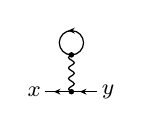
\begin{tikzpicture}[x=0.550cm, y=0.550cm, line width=0.450pt, baseline={([yshift=-0.6ex]0,0)}]
  \draw plot[smooth, tension=0.7] coordinates {(0.000,0.000) (-0.046,0.030) (-0.066,0.061) (-0.046,0.091) (0.000,0.121) (0.046,0.152) (0.066,0.182) (0.046,0.212) (0.000,0.243) (-0.046,0.273) (-0.066,0.304) (-0.046,0.334) (0.000,0.364) (0.046,0.395) (0.066,0.425) (0.046,0.455) (0.000,0.486) (-0.046,0.516) (-0.066,0.546) (-0.046,0.577) (0.000,0.607) (0.046,0.638) (0.066,0.668) (0.046,0.698) (0.000,0.729) (-0.046,0.759) (-0.066,0.789) (-0.046,0.820) (0.000,0.850)};
  \draw (0.000,0.850) arc[start angle=270.000, end angle=630.000, radius=0.280];
  \fill (-0.079,1.410) -- (0.079,1.342) -- (0.028,1.410) -- (0.079,1.478) -- cycle;
  \draw (0.000,0.000) -- (-0.600,0.000);
  \fill (-0.409,0.000) -- (-0.251,-0.068) -- (-0.302,0.000) -- (-0.251,0.068) -- cycle;
  \draw (0.000,0.000) -- (0.600,0.000);
  \fill (0.191,0.000) -- (0.349,-0.068) -- (0.298,0.000) -- (0.349,0.068) -- cycle;
  \fill (0.000,0.000) circle (0.064);
  \fill (0.000,0.850) circle (0.064);
  \node[font=\footnotesize, inner sep=0pt, anchor=0] at (-0.690,0.000) {$x$};
  \node[font=\footnotesize, inner sep=0pt, anchor=180] at (0.690,0.000) {$y$};
\end{tikzpicture}}
\diagramgap
\mbox{$\displaystyle +\,$\,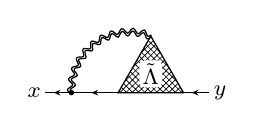
\begin{tikzpicture}[x=0.550cm, y=0.550cm, line width=0.450pt, baseline={([yshift=-0.6ex]0,0)}]
  \draw (-0.753,-0.435) -- (-1.833,-0.435);
  \fill (-1.373,-0.435) -- (-1.214,-0.503) -- (-1.266,-0.435) -- (-1.214,-0.367) -- cycle;
  \draw plot[smooth, tension=0.7] coordinates {(-1.865,-0.436) (-1.907,-0.406) (-1.923,-0.374) (-1.906,-0.342) (-1.865,-0.312) (-1.823,-0.284) (-1.804,-0.255) (-1.818,-0.224) (-1.854,-0.188) (-1.889,-0.151) (-1.899,-0.117) (-1.877,-0.088) (-1.831,-0.066) (-1.785,-0.046) (-1.761,-0.022) (-1.768,0.012) (-1.797,0.053) (-1.825,0.096) (-1.830,0.132) (-1.802,0.156) (-1.753,0.169) (-1.704,0.181) (-1.676,0.201) (-1.678,0.235) (-1.699,0.281) (-1.718,0.328) (-1.716,0.364) (-1.685,0.383) (-1.634,0.387) (-1.584,0.390) (-1.553,0.404) (-1.548,0.438) (-1.561,0.487) (-1.571,0.537) (-1.563,0.572) (-1.529,0.585) (-1.478,0.580) (-1.428,0.573) (-1.395,0.582) (-1.384,0.615) (-1.388,0.665) (-1.389,0.716) (-1.374,0.749) (-1.339,0.755) (-1.290,0.742) (-1.242,0.726) (-1.208,0.729) (-1.191,0.759) (-1.185,0.809) (-1.178,0.859) (-1.157,0.889) (-1.121,0.889) (-1.075,0.867) (-1.031,0.843) (-0.997,0.839) (-0.975,0.866) (-0.961,0.914) (-0.944,0.962) (-0.919,0.988) (-0.883,0.981) (-0.842,0.951) (-0.803,0.920) (-0.770,0.910) (-0.744,0.932) (-0.721,0.977) (-0.696,1.022) (-0.666,1.042) (-0.632,1.029) (-0.597,0.992) (-0.564,0.954) (-0.533,0.939) (-0.504,0.956) (-0.473,0.996) (-0.441,1.035) (-0.408,1.050) (-0.377,1.031) (-0.349,0.988) (-0.323,0.945) (-0.296,0.924) (-0.264,0.936) (-0.226,0.970) (-0.187,1.003) (-0.152,1.011) (-0.125,0.987) (-0.106,0.940) (-0.088,0.893) (-0.065,0.868) (-0.031,0.873) (0.012,0.900)};
  \draw plot[smooth, tension=0.7] coordinates {(-1.801,-0.434) (-1.843,-0.405) (-1.859,-0.374) (-1.842,-0.344) (-1.801,-0.315) (-1.759,-0.288) (-1.741,-0.261) (-1.754,-0.231) (-1.790,-0.197) (-1.825,-0.162) (-1.837,-0.128) (-1.814,-0.102) (-1.769,-0.081) (-1.723,-0.062) (-1.699,-0.039) (-1.707,-0.007) (-1.737,0.033) (-1.765,0.075) (-1.770,0.109) (-1.743,0.132) (-1.694,0.144) (-1.646,0.154) (-1.619,0.173) (-1.621,0.206) (-1.642,0.250) (-1.663,0.296) (-1.661,0.331) (-1.631,0.348) (-1.581,0.351) (-1.532,0.353) (-1.501,0.366) (-1.497,0.399) (-1.511,0.447) (-1.522,0.496) (-1.515,0.530) (-1.482,0.541) (-1.432,0.535) (-1.383,0.528) (-1.351,0.536) (-1.341,0.567) (-1.346,0.616) (-1.349,0.666) (-1.335,0.699) (-1.301,0.704) (-1.253,0.689) (-1.206,0.673) (-1.173,0.675) (-1.158,0.704) (-1.153,0.754) (-1.147,0.803) (-1.128,0.833) (-1.093,0.832) (-1.048,0.809) (-1.005,0.784) (-0.972,0.780) (-0.952,0.806) (-0.939,0.854) (-0.924,0.902) (-0.900,0.927) (-0.865,0.920) (-0.826,0.889) (-0.788,0.857) (-0.756,0.847) (-0.732,0.869) (-0.710,0.914) (-0.686,0.958) (-0.658,0.979) (-0.626,0.966) (-0.592,0.928) (-0.561,0.890) (-0.532,0.875) (-0.503,0.892) (-0.474,0.932) (-0.443,0.971) (-0.411,0.986) (-0.382,0.968) (-0.356,0.925) (-0.332,0.882) (-0.306,0.861) (-0.275,0.873) (-0.239,0.907) (-0.201,0.940) (-0.167,0.949) (-0.142,0.926) (-0.124,0.879) (-0.108,0.832) (-0.086,0.807) (-0.053,0.813) (-0.012,0.840)};
  \draw (0.000,0.000) -- (-0.753,-0.435);
  \draw (0.000,0.000) -- (0.753,-0.435);
  \draw (0.000,0.000) -- (0.000,0.870);
  \draw (-1.833,-0.435) -- (-2.433,-0.435);
  \fill (-2.243,-0.435) -- (-2.084,-0.503) -- (-2.136,-0.435) -- (-2.084,-0.367) -- cycle;
  \draw (0.753,-0.435) -- (1.353,-0.435);
  \fill (0.944,-0.435) -- (1.103,-0.503) -- (1.051,-0.435) -- (1.103,-0.367) -- cycle;
  \fill[white] (-0.753,-0.435) -- (0.753,-0.435) -- (0.000,0.870) -- cycle;
  \draw[line width=0.248pt] (-0.029,0.819) -- (0.008,0.856) (-0.223,0.485) -- (0.060,0.767) (-0.416,0.150) -- (0.111,0.677) (-0.609,-0.185) -- (0.163,0.587) (-0.718,-0.435) -- (0.215,0.498) (-0.576,-0.435) -- (0.267,0.408) (-0.435,-0.435) -- (0.318,0.318) (-0.294,-0.435) -- (0.370,0.229) (-0.152,-0.435) -- (0.422,0.139) (-0.011,-0.435) -- (0.474,0.049) (0.131,-0.435) -- (0.525,-0.040) (0.272,-0.435) -- (0.577,-0.130) (0.414,-0.435) -- (0.629,-0.220) (0.555,-0.435) -- (0.681,-0.309) (0.696,-0.435) -- (0.733,-0.399) (-0.733,-0.399) -- (-0.696,-0.435) (-0.681,-0.309) -- (-0.555,-0.435) (-0.629,-0.220) -- (-0.414,-0.435) (-0.577,-0.130) -- (-0.272,-0.435) (-0.525,-0.040) -- (-0.131,-0.435) (-0.474,0.049) -- (0.011,-0.435) (-0.422,0.139) -- (0.152,-0.435) (-0.370,0.229) -- (0.294,-0.435) (-0.318,0.318) -- (0.435,-0.435) (-0.267,0.408) -- (0.576,-0.435) (-0.215,0.498) -- (0.718,-0.435) (-0.163,0.587) -- (0.609,-0.185) (-0.111,0.677) -- (0.416,0.150) (-0.060,0.767) -- (0.223,0.485) (-0.008,0.856) -- (0.029,0.819);
  \begin{scope}
  \clip (-0.753,-0.435) -- (0.753,-0.435) -- (0.000,0.870) -- cycle;
  \node[font=\footnotesize, inner sep=1.2pt, fill=white, rounded corners=2pt] at (0.000,0.000) {$\tilde\Lambda$};
  \end{scope}
  \draw (-0.753,-0.435) -- (0.753,-0.435) -- (0.000,0.870) -- cycle;
  \fill (-1.833,-0.435) circle (0.064);
  \node[font=\footnotesize, inner sep=0pt, anchor=0] at (-2.523,-0.435) {$x$};
  \node[font=\footnotesize, inner sep=0pt, anchor=180] at (1.443,-0.435) {$y$};
\end{tikzpicture}}
